\documentclass[paper=A3,landscape,14pt]{scrartcl}
\usepackage{graphicx}
\usepackage{amsbsy}
\thispagestyle{empty}
\usepackage{geometry}
\geometry{tmargin=2cm,bmargin=2cm,lmargin=2cm,rmargin=2cm}
\begin{document}

\Huge

\begin{center}
  \scalebox{2}{\textsf{\textbf{Die Kreiszahl~$\boldsymbol{\pi}$, eine transzendente Zahl}}}
  \vspace{3em}

  \scalebox{1.42}{141 592 6535 897 932 3846 264 338 3279 502 884 1971 693 993 7510}

  \scalebox{1.42}{582 097 4944 592 307 8164 062 862 0899 862 803 4825 342 117 0679}

  \scalebox{1.42}{821 480 8651 328 230 6647 093 844 6095 505 822 3172 535 940 8128}

  \scalebox{1.42}{481 117 4502 841 027 0193 852 110 5559 644 622 9489 549 303 8196}

  \scalebox{1.42}{442 881 0975 665 933 4461 284 756 4823 378 678 3165 271 201 9091}

  \scalebox{1.42}{456 485 6692 346 034 8610 454 326 6482 133 936 0726 024 914 1273}

  \scalebox{1.42}{724 587 0066 063 155 8817 488 152 0920 962 829 2540 917 153 6436}

  \scalebox{1.42}{789 259 0360 011 330 5305 488 204 6652 138 414 6951 941 511 6094}

  \scalebox{1.42}{330 572 7036 575 959 1953 092 186 1173 819 326 1179 310 511 8548}

  \scalebox{1.42}{074 462 3799 627 495 6735 188 575 2724 891 227 9381 830 119 4912}

  \vfill
  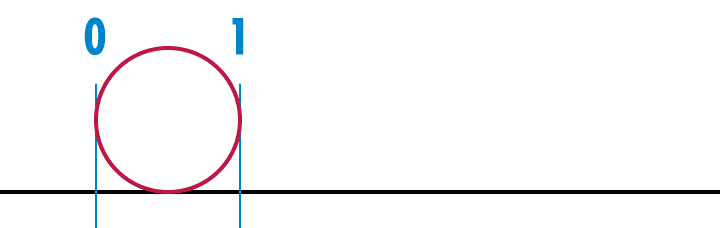
\includegraphics[scale=0.308]{pi-1}\hfill%
  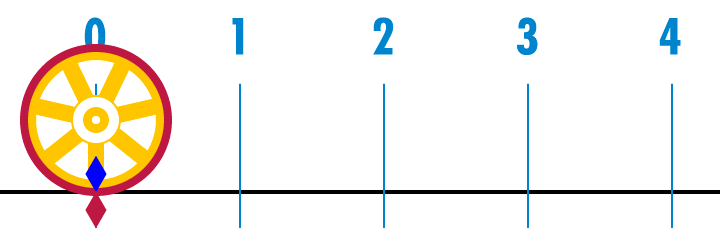
\includegraphics[scale=0.308]{pi-2}\hfill%
  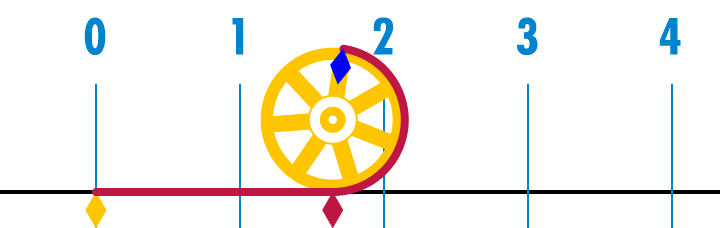
\includegraphics[scale=0.308]{pi-3}\hfill%
  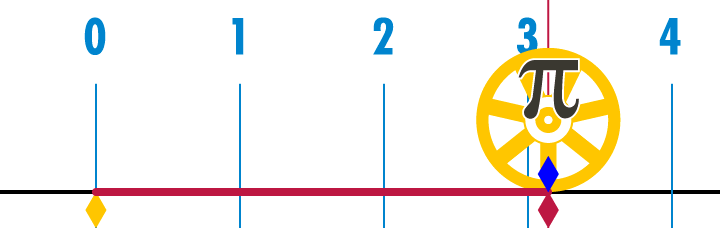
\includegraphics[scale=0.308]{pi-4}
\end{center}

\end{document}
